\documentclass{beamer}
\setbeameroption{show notes}
\setbeamerfont{framesubtitle}{size=\normalfont\large}
\setbeamertemplate{footline}[frame number]

\usepackage[utf8]{inputenc}
\usepackage[T1]{fontenc}
% \usepackage[ngerman]{babel}

\title{\\\emph{A Theory of Type Qualifiers}\\ \small{}by Jeffrey S. Foster, Manuel Fähndrich, Alexander Aiken}
\author{Paper presentation by\\Georg Schmid and Karl Samuel Grütter}
\date{May 20, 2015}

\usepackage{amssymb}
\usepackage{parskip}
\usepackage{listings}
\usepackage{graphicx}

\usepackage{todonotes}
\let\todox\todo
\renewcommand\todo[1]{\todox[inline]{#1}}

\begin{document}
\maketitle

\begin{frame}{Overview}
  \begin{itemize}
  \item Many languages support a range of \emph{type qualifiers} -- they enable a simple, yet useful form of subtyping.

  \item Authors present a framework for adding type qualifiers to $\lambda$-calculi.

  \item In particular, they show how to
    \begin{itemize}
    \item extend the typing rules, and
    \item support type inference --
    \item even in the polymorphic case.
    \end{itemize}
  \end{itemize}
\end{frame}


\defverbatim{\lstcduplicateprocs}{%
\begin{lstlisting}[language=C,frame=single,belowskip=- \medskipamount]
int *id1(int *x) { return x; }
const int *id2(const int *x) { return x; }
\end{lstlisting}}

\begin{frame}[fragile]{Motivation}
  \begin{itemize}
  \item Paper's presentation is closely tied to \textsc{const} qualifier in C

  \item[$\Rightarrow$] Use-case: Analyze C sources and infer additional \textsc{const} qualifiers

  \item<2->
    This rectifies one particular peculiarity of C's type system:
    % \vspace{1em}
    \lstcduplicateprocs
    $\rightarrow$ Inference of \textsc{const} qualifiers removes need for multiple versions of same procedure
    \todo{Replace with better example?}
  \end{itemize}
\end{frame}

\note[itemize]{%
  \item\emph{Q:} What does \textsc{const} in C mean?}


\begin{frame}{Preliminaries}{Basic syntax / notation / definitions}
  \begin{itemize}
  \item type constructor, $\mathit{Typ}$ (paper\_typ.png), type environment
  \item framework allows mapping of source lang to lang with qualifiers; paper's source language (paper\_sourcelang)
  \item qualifiers, pos./neg. (paper\_negposqualifier), negation of a qualifier
  \item qualifier lattice (paper\_qualifierlattice\_\{def,sample\})
  \item intuition on qualifier lattice: losing ``information''/capabilites as we move up the lattice
  \end{itemize}
  \todo{Split into multiple slides and expand}
\end{frame}

\note[itemize]{%
  \item\emph{Q:} What is a two-point lattice?\\
  \item\emph{Q:} What is $\bot$ of this lattice? What is $\top$?\\
  \item\emph{Q:} ``Subset contradiction'' wrt.\ $\tau \subseteq \text{const}\ \tau$ (cf.\ dual notation as negative qualifier ``writable'' / consider \textsc{const} as ``read-only'' / rewrite as ``ConstInt'' $\geq$ ``NormalInt'' class hierarchy)}


\begin{frame}{Qualified types}
  \begin{itemize}
  \item $\mathit{QTyp}$ (paper\_qtyp), resulting concrete types wrt.\ sample lang
  \item subtyping rules (paper\_samplelang\_subtypingrules)
  \end{itemize}
\end{frame}


\begin{frame}{Qualifier annotations and assertions}
  \begin{itemize}
  \item purpose of annotations: support type inference -- problem: which type qualifier to choose for a given inferred type?
  \item ``qualifier annotations'' are added to the source language as a syntactic helper -- together with the resp.\ typing rule, qualifiers can only increase monotonically (``give up capabilities'')
  \item additionally, dual notion of ``qualifier assertions''
  \item source language extended (paper\_qualifierannass\_syntax), both enforce $e$'s top-level qualifier $Q_e$ to be upper-bounded by $l$, i.e.\ $Q_e \sqsubseteq l$ (-> Q)
  \item cf.\ typing rules (paper\_samplelang\_annasstyping)
  \end{itemize}
  \todo{Split into multiple slides and expand}
\end{frame}

\note[itemize]{%
  \item\emph{Q:} What's the difference between assertions and annotations? (Hint: Show typing rules)\\
  \item\emph{Q/Follow-up:} What's the difference between Q and l?}


\begin{frame}{Qualified type systems}
  \begin{center}\Large
  \begin{tabular}{l c r}
    $A \vdash e : \tau$ & $\Rightarrow$ & $A \vdash e : \rho$
  \end{tabular}
  \end{center}

  \vspace{1em}
  \large
  Extending the source language's type checking system with qualified types leads to a \emph{qualified type system}.
\end{frame}

\begin{frame}{Qualified type systems}{Typing rules of sample language (1)}
  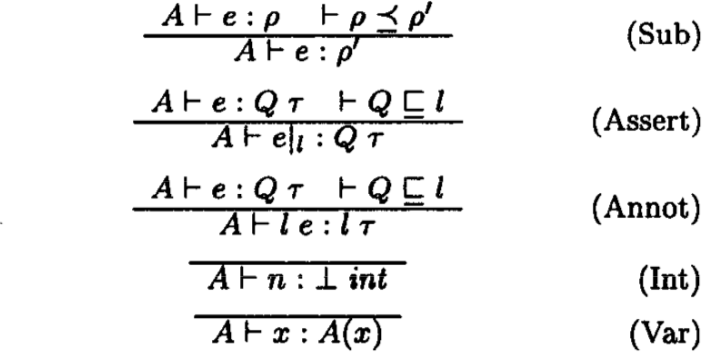
\includegraphics[scale=0.4]{paper_samplelang_typingrules1.png}
\end{frame}

\note[itemize]{%
  \item Discuss unrestricted type qualifier $Q$ in premises.
  \item Discuss how terminal expressions are assigned type qualifier $\bot$.}

\begin{frame}{Qualified type systems}{Typing rules of sample language (2)}
  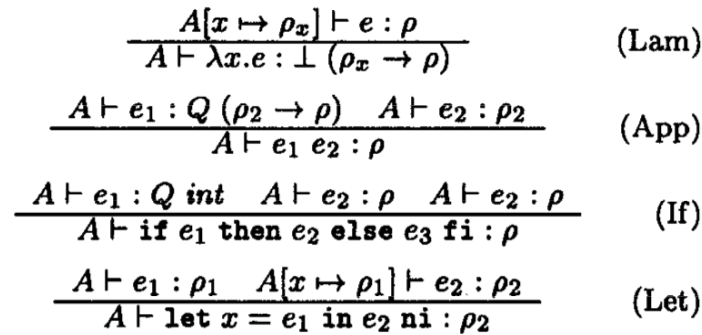
\includegraphics[scale=0.4]{paper_samplelang_typingrules2.png}
\end{frame}

\note[itemize]{\item\emph{Q:} Ad $(\text{App})$. What role do qualifiers on abstractions play in this paper?}


\begin{frame}{Qualified type systems}{Correspondence}
  \begin{itemize}
  \item type qualifiers should only refine type information,\\ but \emph{not} modify type structure
  \item[$\Rightarrow$] correspondence of the original and resp.\ qualified type system
  \item<2-> Helpers:\\
    \begin{description}
    \item[$\mathit{Typ} \rightarrow \mathit{QTyp}$:] $\text{strip}(\cdot)$ \ldots eliminates qualifiers \& annotations\\
      \visible<3->{\vspace{0.5em}\hspace{-4em}
        $\text{strip}(\,\overline{\bot(\text{const}\ \text{int} \to \text{nonzero}\ \text{int})}\,) =
         \overline{(\text{int} \to \text{int})}$
        }
    \item[$\mathit{QTyp} \rightarrow \mathit{Typ}$:] $\bot(\cdot)$ \ldots introduces $\bot$ qualifiers \& annotations\\
      \visible<4->{\vspace{0.5em}\hspace{-4em}
        $\bot(\,\overline{(\text{int} \to \text{int})}\,) =
          \overline{\bot(\bot\ \text{int} \to \bot\ \text{int})}$
        }
    \end{description}
  % \item[]<2->
  %   \begin{center}
  %   \vspace{1em}
  %   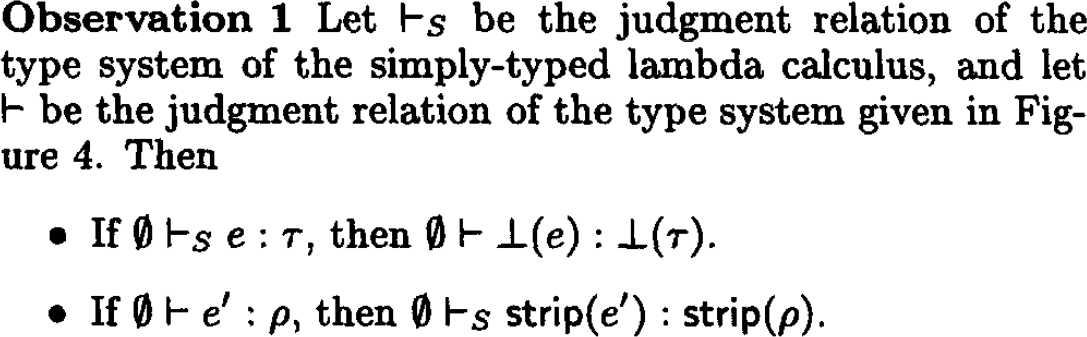
\includegraphics[scale=0.25]{paper_observation1.png}
  %   \end{center}
    \visible<4->{\todo{Verify that this is line with the paper's definition of $\bot(\cdot)$.}
      \todo{Improve readability.}}
  \end{itemize}
\end{frame}

% \note[itemize]{%
%   \item Discuss definition of $\bot(\cdot)$ and $\text{strip}(\cdot)$.}

\begin{frame}{Qualified type systems}{Correspondence (ctd.)}
  \begin{center}
  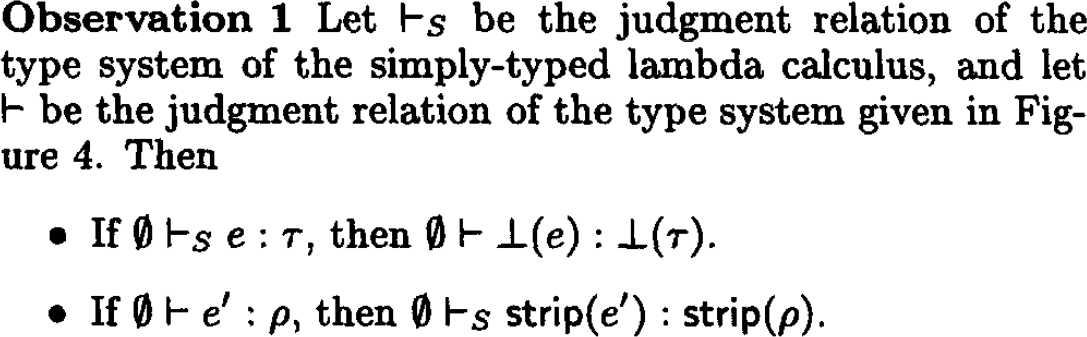
\includegraphics[scale=0.25]{paper_observation1.png}
  \end{center}
\end{frame}

\note[itemize]{%
  \item\emph{Q:} Ad $\bot(\cdot)$. Could we use $\top$ instead? Any other qualifier?\\\quad$\rightarrow$ Here, the choice of qualifier is unimportant.}


\begin{frame}{Qualifier semantics}
  \begin{itemize}
  \item Restrictions on usage of qualifiers can be expressed
    \begin{enumerate}[a)]
    % \item using qualifier assertions (injected during a preprocessing step of programs), or
    \item using qualifier assertions ($\rightarrow$ program transformation), or
    \item by modifying typing rules.
    \end{enumerate}
  \item Arbitrary modifications may render the type system unsound!
  \end{itemize}
\end{frame}

\begin{frame}{Qualifier semantics}{\textsc{const} example}
  \begin{itemize}
  \item Let's encode the semantics of a \textsc{const} qualifier!
  \item<2-> Only makes sense in presence of \emph{references}:
    \begin{center}
    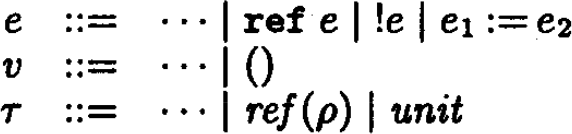
\includegraphics[scale=0.3]{paper_ref_syntax.png}
    \end{center}
  \end{itemize}
\end{frame}

\note{\emph{Q:} Why do they introduce unit / $()$? (Hint: Why only along with references?)}

\begin{frame}{Qualifier semantics}{\textsc{const} example (2)}
  \begin{itemize}
  \item A first attempt:
    \begin{center}
    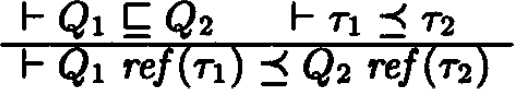
\includegraphics[scale=0.29]{paper_ref_unsound.png}
    \end{center}
  \item<2-> Unsound in the presence of subtyping!
    \begin{center}
    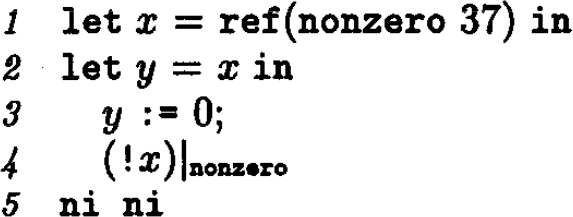
\includegraphics[scale=0.3]{paper_ref_unsoundsample.png}
    \end{center}
  \item<3->[$\Rightarrow$] Note that lines 3 and 4 type check, e.g.\
    \begin{minipage}[t]{0.3\textwidth}
    \begin{tabbing}
    \=\#3: \=$A[x, y \mapsto \bot\,\text{ref nonzero int}]\,\vdash y : \neg\text{nonzero int}$\quad \=\small(by $(\text{Sub})$)\\
    \>\#4: \>$A[x, y \mapsto \bot\,\text{ref nonzero int}]\,\vdash\ !x : \text{nonzero int}$ \>\small(unchanged)
    \end{tabbing}
    \end{minipage}
    \todo{Should introduce qualifier negation for this.}
  \end{itemize}
\end{frame}

\begin{frame}{Qualifier semantics}{\textsc{const} example (3)}
  \begin{itemize}
  \item Requiring refs' argument type to be invariant, fixes our problem.
    \begin{center}
    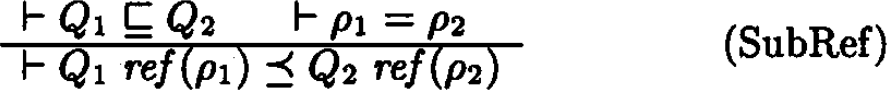
\includegraphics[scale=0.29]{paper_ref_sound.png}
    \end{center}
  \item<2-> Generally, subtyping rules of the form
    \begin{center}
    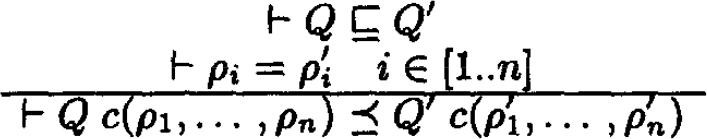
\includegraphics[scale=0.3]{paper_subtypingrule_general.png}
    \end{center}
    are sound.
  \end{itemize}
\end{frame}

\begin{frame}{Qualifier semantics}{\textsc{const} example (4)}
  \begin{itemize}
  \item How do we enforce the semantics of \textsc{const}?
  \item<2-> As mentioned before, there are two ways to encode such restrictions:
    \begin{enumerate}[a)]
    \item<2-> Program transformation:\\ Replace every assignment $e\,=\,e_1\!:=\!e_2$ by $e\!\mid_{\neg\text{const}}$.
    \item<3-> Modify the relevant typing rule(s):\\
      \begin{center}
      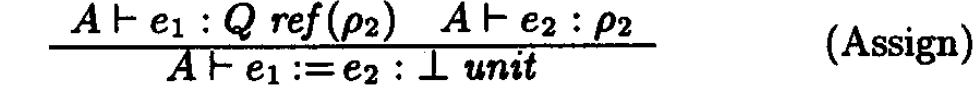
\includegraphics[scale=0.25]{paper_assign_original.png}\\
      \vspace{0.5em}{\Huge $\Downarrow$}\hspace{5.8em}\vspace{0.5em}\\
      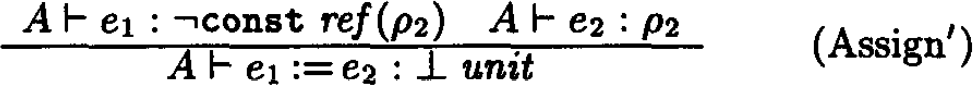
\includegraphics[scale=0.25]{paper_assign_adapted.png}
      \end{center}
    \end{enumerate}
  % \item<2-> Generally, subtyping rules of the form
  %   \begin{center}
  %   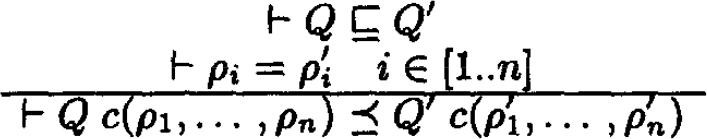
\includegraphics[scale=0.3]{paper_subtypingrule_general.png}
  %   \end{center}
  %   are sound.
  \end{itemize}
\end{frame}


\end{document}